% from hyperparameter tuning (selecting for highest accuracy on the dev set)
% - [17:04:30] Best Linear SVM params: {'C': 1.0, 'loss': 'hinge'} (Dev Accuracy: 0.9165)
% - [17:03:58] Best Logistic Regression params: {'C': 1.0} (Dev Accuracy: 0.9155)




% linear svm (test) classification report
\begin{table}[h]
\centering
\begin{tabular}{lcccc}
\toprule
 & \textbf{Precision} & \textbf{Recall} & \textbf{F1-Score} & \textbf{Support} \\
\midrule
1            & 0.94 & 0.90 & 0.92 & 1900 \\
2            & 0.95 & 0.98 & 0.97 & 1900 \\
3            & 0.89 & 0.88 & 0.89 & 1900 \\
4            & 0.89 & 0.90 & 0.90 & 1900 \\
\midrule
Accuracy     & \multicolumn{2}{c}{} & 0.92 & 7600 \\
Macro avg    & 0.92 & 0.92 & 0.92 & 7600 \\
Weighted avg & 0.92 & 0.92 & 0.92 & 7600 \\
\bottomrule
\end{tabular}
\caption{Classification Report}
\end{table}

% linear svm (test) confusion matrix
\begin{figure}[H]
    \centering
    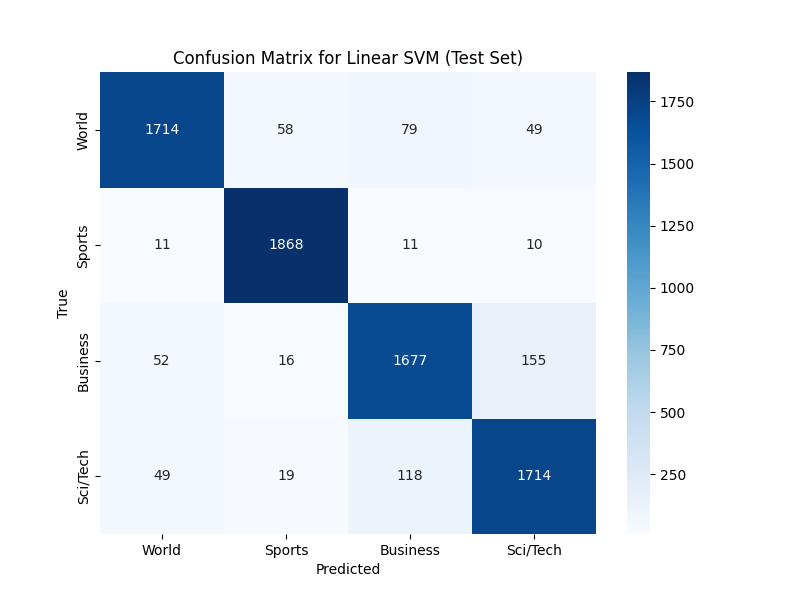
\includegraphics[width=0.5\textwidth]{../figures/linear_svm_test_confusion_matrix.png}
    \caption{Confusion Matrix for Linear SVM on Test Set}
\end{figure}


% logistic regression (test) classification report
\begin{table}[h]
\centering
\begin{tabular}{lcccc}
\toprule
 & \textbf{Precision} & \textbf{Recall} & \textbf{F1-Score} & \textbf{Support} \\
\midrule
1            & 0.93 & 0.91 & 0.92 & 1900 \\
2            & 0.95 & 0.98 & 0.96 & 1900 \\
3            & 0.88 & 0.89 & 0.88 & 1900 \\
4            & 0.89 & 0.89 & 0.89 & 1900 \\
\midrule
Accuracy     & \multicolumn{2}{c}{} & 0.91 & 7600 \\
Macro avg    & 0.91 & 0.91 & 0.91 & 7600 \\
Weighted avg & 0.91 & 0.91 & 0.91 & 7600 \\
\bottomrule
\end{tabular}
\caption{Classification Report}
\end{table}

% logistic regression (test) confusion matrix
\begin{figure}[H]
    \centering
    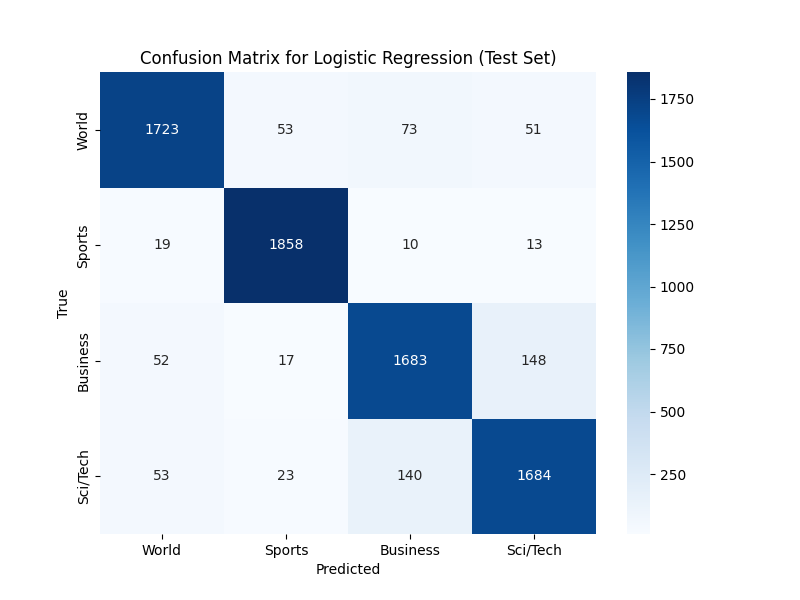
\includegraphics[width=0.5\textwidth]{../figures/logistic_regression_test_confusion_matrix.png}
    \caption{Confusion Matrix for Logistic Regression on Test Set}
\end{figure}


% table of comparison of accuracy and macro-F1 for linear svm and logistic regression on the test set
\begin{table}[h]
\centering
\begin{tabular}{lcc}
\toprule
\textbf{Model} & \textbf{Accuracy} & \textbf{Macro-F1} \\
\midrule
Linear SVM & \textbf{0.92} & \textbf{0.92} \\
Logistic Regression & 0.91 & 0.91 \\
\bottomrule
\end{tabular}
\caption{Comparison of Accuracy and Macro-F1 for Linear SVM and Logistic Regression on Test Set}
\end{table}

% mention that the linear SVM performs slightly better than logistic regression on both accuracy and macro-F1, but the difference is not very large (e.g., 0.01 in accuracy and macro-F1)

% they also perform the same type of errors, as seen in the confusion matrices (e.g., both models get confused between sci/tech and business, which is reflected in the confusion matrices where there are more misclassifications between these classes than between the others)

% mention that for both models, sport is the easiest class to classify (highest precision, recall, and F1-score), while sci/tech is the hardest (lowest precision, recall, and F1-score), which is also reflected in the confusion matrices where there are more misclassifications involving sci/tech than the other classes